% !TEX root = Projektdokumentation.tex
% \section{Anhang}
% \subsection{Schritt-für-Schritt Anleitung}
% \label{app:Anleitung}
% gesetzt in der pagecommand-Option von \includepdf, damit die erste PDF-Seite die richtigen Header bekommt
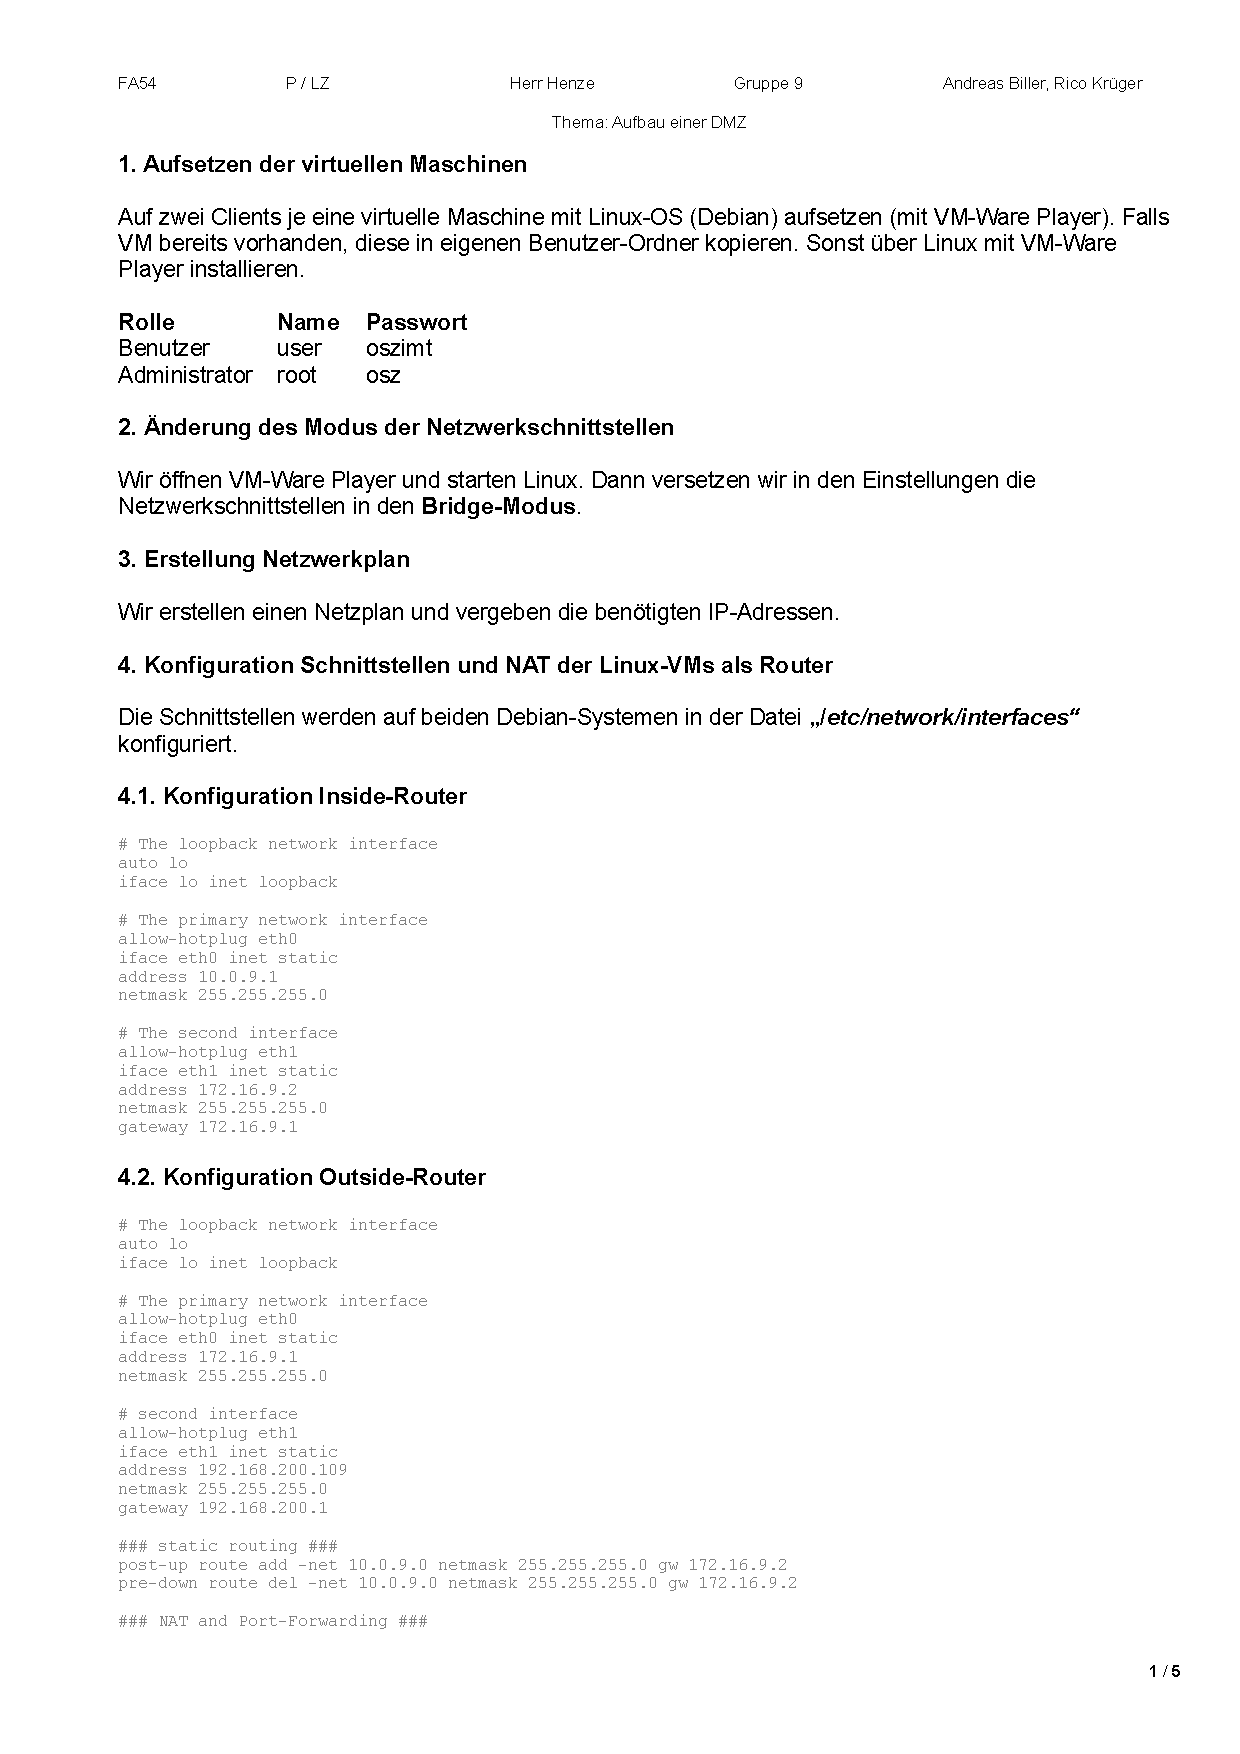
\includepdf[scale=0.8,clip,trim=0cm 0cm 0cm 0cm,offset=0 -2cm,pages={1},pagecommand={\section{Anhang}\subsection{Schritt-für-Schritt Anleitung}\label{app:Anleitung}}]{AufbauEinerDMZ.pdf}
\includepdf[scale=0.85,clip,trim=0cm 0cm 0cm 0cm,offset=0 -0.5cm,pages={2-5},pagecommand={}]{AufbauEinerDMZ.pdf}
\clearpage

\subsection{Lastenheft}
\label{app:Lastenheft}
Es folgt unser Lastenheft mit Fokus auf den Anforderungen:

Die Umsetzung muss folgende Anforderungen erfüllen: 
\begin{enumerate}[itemsep=0em,partopsep=0em,parsep=0em,topsep=0em]
\item DMZ
	\begin{enumerate}
	\item Die DMZ soll aus zwei virtuellen, zu Routern konfigurierten Linux-Distributionen bestehen, welch die Netze INSIDE, OUTSIDE und das DMZ-Netz miteinander verbinden. 
	\item Die Router sollen entsprechend des Netzplanes eingerichtet und konfiguriert werden.
	\item Die DMZ soll Zugriffe auf den Webserver erlauben, aber Zugriffe auf das INSIDE-Netz verhindern. Hierzu soll auf dem Outside-Router NAT, Portforwarding und eine Firewall laufen.
    \item Die Router sollen nur vom Client-Rechner her fernadministrierbar sein.
	\end{enumerate}
\item Client-Rechner
\begin{enumerate}
    \item Der Client-Rechner im INSIDE-Netz nutzt das Betriebssystem Windows.
    \item Der Webserver soll eine Webseite mit dem aktuellen Stand der Gruppe anzeigen.    
\end{enumerate}
\item Webserver
\begin{enumerate}
    \item Der Webserver nutzt das Betriebssystem Windows. Er wird über das Tool Mini-Webserver vom Auftraggeber bereitgestellt.
    \item Der Webserver im DMZ-Netz muss vom OUTSIDE-Netz über Port 80 erreichbar sein. Hierzu soll auf dem Outside-Router NAT und Port-Forwarding eingerichtet werden.
    \item Der Webserver soll eine Webseite mit dem aktuellen Stand der Gruppe anzeigen.    
\end{enumerate}
\item Firewall
\begin{enumerate}
    \item Die Firewall soll den Webserver in der DMZ über Port 80 erreichbar sein lassen.
    \item Die Firewall soll SSH nur vom Admin-PC zulassen.
    \item Die Firewall soll ICMP zulassen.
    \item Die Firewall soll DNS zulassen.
    \item Die Firewall soll RDP zulassen.
    \item Die Firewall soll per Script an- und ausschaltbar sein. Hierzu muss an diversen Stellen per Script die Linux-Systemkonfiguration verändert werden
\end{enumerate}
\item Sonstige Anforderungen
	\begin{enumerate}
	\item Das Projekt soll unter Berücksichtigung der von der IHK ausgegebenen Richtlinien für eine Projektdokumentation dokumentiert werden.
    \item Es soll ein logischer Netzplan in Papierform erstellt und der Dokumentation angefügt werden.
	\item Pro Person soll ein ausführliches Kompetenzportfolio erstellt werden, welches einen kritischen Überblick über unsere individuellen Kompetenzstände vor, während und nach dem Projekt liefert. Diese sollen der Dokumentation angehängt werden.
	\item Die Funktionalität der Firewall soll getestet und die Ergebnisse in zwei Testprotokollen festgehalten werden. Diese sind der Dokumentation anzuhängen.
	\end{enumerate}
\end{enumerate}


\subsection{Pflichtenheft}
\label{app:Pflichtenheft}

Unser aus den Anforderungen des Lastenheftes erstelltes Pflichtenheft:

\begin{enumerate}[itemsep=0em,partopsep=0em,parsep=0em,topsep=0em]
\item Musskriterien % Wikipedia: für das Produkt unabdingbare Leistungen, die in jedem Fall erfüllt werden müssen
    \begin{enumerate}
    \item Das DMZ-Netz erhält die Netzmaske 172.16.9.0/24
    \item Das intere Netz erhält die Netzmaske 10.0.9.0/24
    \item Die öffentliche Schnittstelle des Outside-Router erhält die IP 192.168.200.109
    \item Der Outside-Router erhält als Standard-Gateway die IP 192.168.200.1
    \item Der Outside-Router erhält eine statische Route für das interne und DMZ-Netz
    \item Der Inside-Router erhält als Standard-Gateway das Interface des Outside-Routers, welches in die DMZ zeigt
    \item Der Webserver ist über die öffentliche IP des Outside-Routers über HTTP/S von außen erreichbar
    \item Der Webserver ist über die lokale IP 172.16.9.3 über HTTP/S aus dem internen Netzwerk erreichbar
    \item Die Router und Windows-Clients bekommen als DNS-Server die IPs 192.168.95.40 und 192.168.95.41
    \item Die Router und Windows-Clients bekommen als NTP-Server die IP 192.168.200.1
    \item Die Firewall verhindert unrechtmäßigen Datentransfer zwischen den Netzen und auf den Routern
    \item Der Admin-PC mit der IP 10.0.9.2 ist berechtigt mittels SSH auf die Router zuzugreifen	
    \end{enumerate}
\item Kannkriterien
    \begin{enumerate}
    \item Die Firewall lässt sich mit den Optionen "start" und "stop" an- bzw.\ ausschalten
    \item Die Firewall-Scripts der Router befinden sich im Verzeichnis /root/bin
    \item Die Veränderung der Firewall-Konfiguration befindet sich jeweils im Verzeichnis /var/log/firewall
    \item Der Admin-PC mit der IP 10.0.9.2 ist berechtigt mittels RDP auf den Webserver zuzugreifen
    \end{enumerate}
\end{enumerate}
	
\clearpage

\subsection{Netzpläne}
\label{app:Netzplan}
Der Netzplan unserer DMZ in der Projektumgebung im Labor 3.1.01:
\begin{figure}[htb]
\centering
\includegraphicsKeepAspectRatio{PLZNetzplanProjektumgebung.png}{0.8}
\caption{Netzplan der DMZ in Raum 3.1.01 (Arbeitsgruppe 9)}
\end{figure}

Der Netzplan unserer DMZ in der virtualisierten Testumgebung:
\begin{figure}[htb]
    \centering
    \includegraphicsKeepAspectRatio{PLZNetzplanTestumgebung.png}{0.8}
    \caption{Netzplan der erweiterten DMZ in unserer virtuellen Testumgebung}
\end{figure}
\clearpage

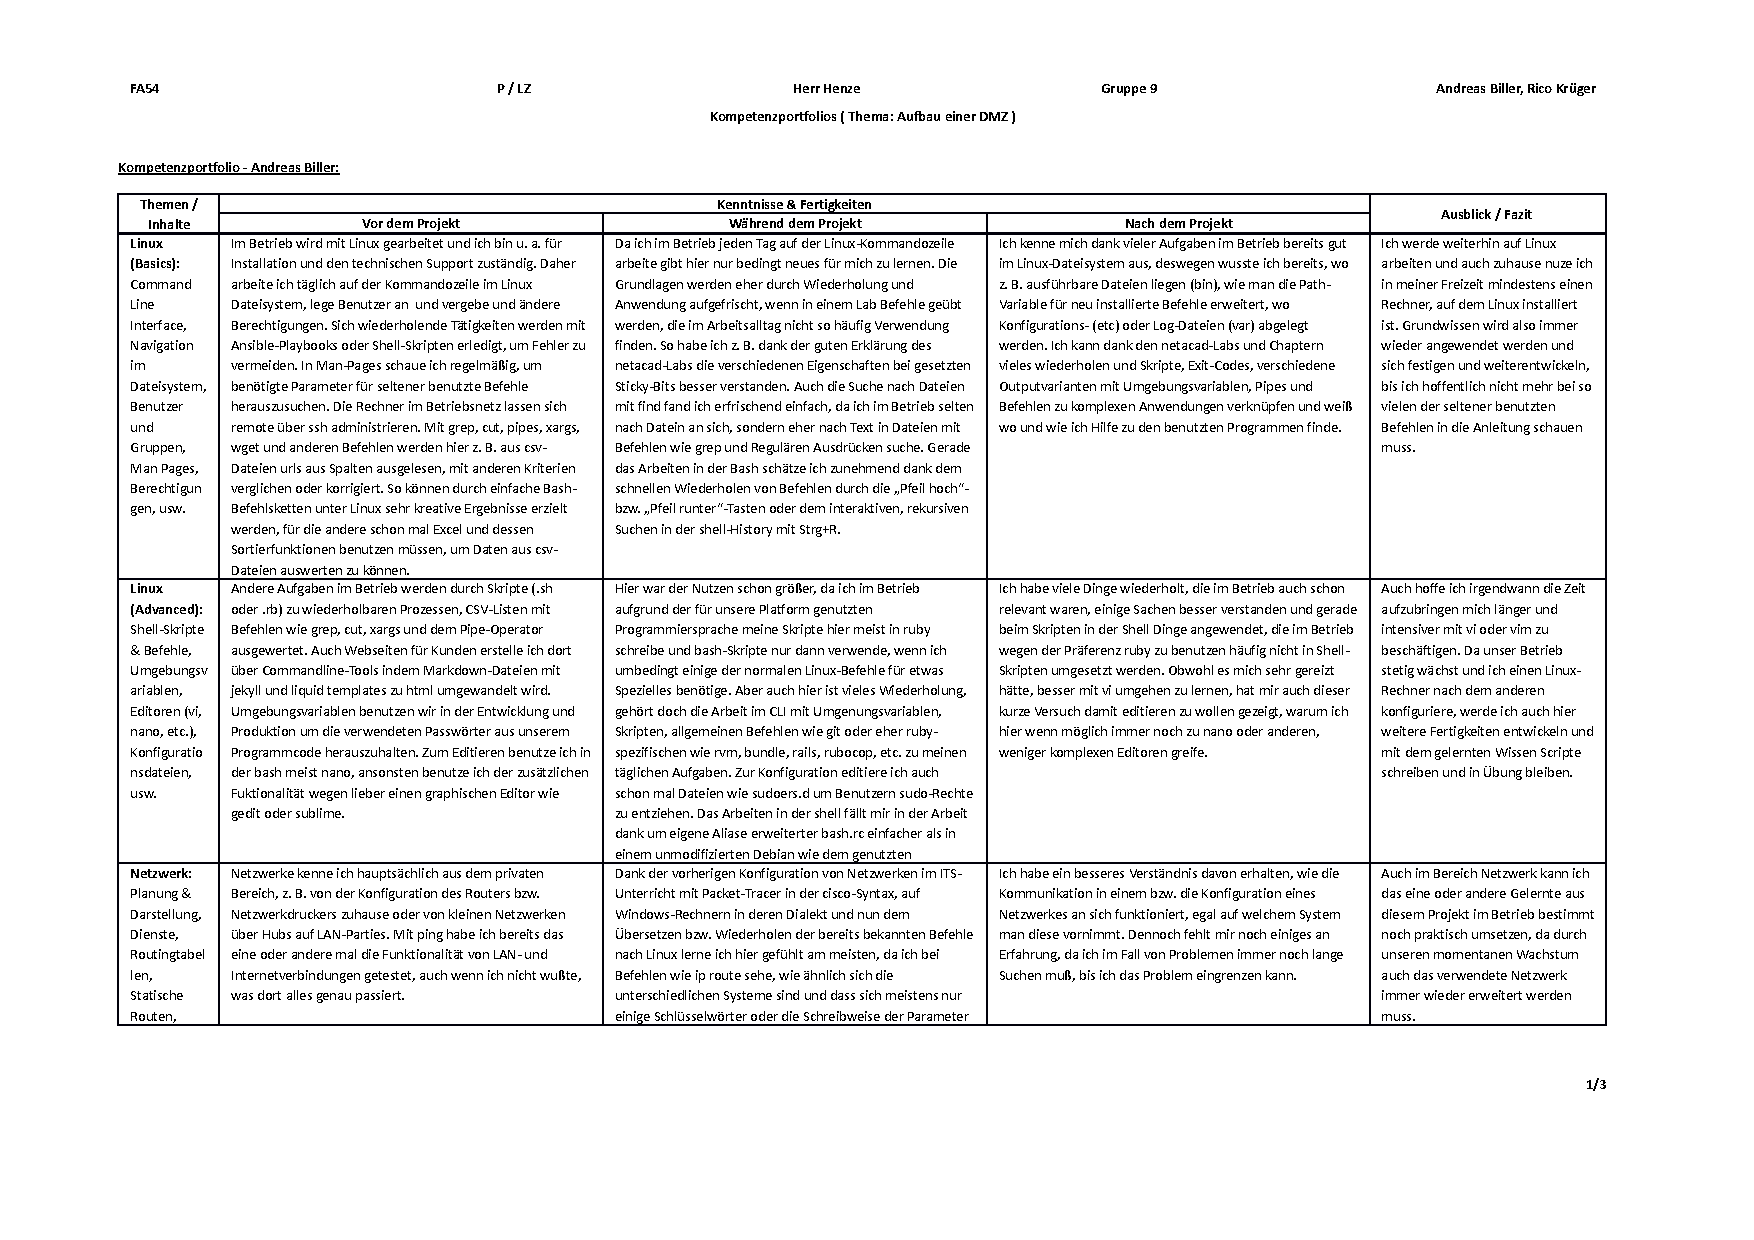
\includepdf[scale=0.925,clip,trim=0cm 0cm 0cm 0cm,offset=0.7cm -1cm,landscape=true,pages={1},pagecommand={\subsection{Kompetenzportfolios}\label{app:Kompetenz}}]{Kompetenzportfolios.pdf}
\includepdf[scale=0.95,clip,trim=0cm 0cm 0cm 0cm,offset=0.5cm -0.4cm,landscape=true,pages={2-3},pagecommand={}]{Kompetenzportfolios.pdf}
\clearpage

\section{Testdokumentation}
\label{app:Test}

\begin{table}[!ht]
    \tabelleAnhang{Systeminformation}{tab:Systeminformation}{Systeminformation.tex}
    \caption{Hardwaredetails des Testsystems}
    \label{tab:tabletestsystem}
\end{table}

\subsection{Aufbau der Testumgebung}
\label{app:testaufbau}
Die zur Umsetzung dieses Kapitels benötigten Informationen entstammen unter anderem den hilfreichen Artikeln folgender Webseiten: \cite{networkdriverhacking}

\subsubsection{Implementierung der Virtuellen Maschinen}
Im Server-Manager fügen wir über \textit{Verwalten > Rollen und Features hinzufügen} den Hyper-V-Manager hinzu indem wir dem Assistenten folgen. Dieser gestattet es virtuelle Maschinen und Netzwerke zu installieren.
Als nächstes wird eine neue virtuelle Linux (Debian 7.1)  Maschine (Generation 1) aus einem Image erstellt. Dies geschieht mit Hilfe eines Assistenten. Sie bekommt einen virtuellen Prozessor und 1 \ac{GB} Arbeitsspeicher. Des weiteren wird bei der Installation eine 5 \ac{GB} große Festplatte für die Maschine erstellt und ihr zugewiesen. Als virtuellen Switch weisen wir ihr vorläufig den Netzwerkadapter des Hosts zu. Somit besitzt unsere Linux-\ac{VM} Internet. Um sie zu installieren, startet man nun die Maschine und verbindet sich zu ihr. Danach folgt man wie gewohnt den Installationsschritten wie bei einer physischen Maschine. Danach installieren wir den \ac{NTP}-Service. Ist die Grundkonfiguration fertig, wird die Maschine ausgeschaltet.
Die Installation der Windows 7 \ac{VM} erfolgt analog zu die der Linux \ac{VM}. Wir vergeben jedoch 4 \ac{GB} \ac{RAM} und erstellen eine mindestens 30 \ac{GB} große virtuelle Festplatte. Nach der Installation wird die Firewall wie in \nameref{sec:Implementierungsphase} eingerichtet. Zusätzlich werden noch nützliche Software wie putty oder winscp heruntergeladen.
Nach der Grundkonfiguration der beiden \ac{VM}s können diese nun dupliziert werden. Dazu muss man die virtuelle Maschine erst exportieren, um sie danach wieder zu importieren. Beim Import sollte man darauf achten, dass man \textit{eine neue eindeutige \ac{ID} } erstellt. Nachdem starten der importierten Maschine wird als erstes der Hostname geändert, um sie von der Originalen zu unterscheiden und um \ac{DNS}-Konflikte zu vermeiden.

\subsubsection{Implementierung des virtuellen Netzwerkes}
Virtuelle Netzwerke werden über das Hinzufügen virtueller Switche an den Netzwerkadaptern der virtuellen Maschine erstellt. Auf diesen lassen sich auch \ac{VLAN}s einrichten.
Die Installation eines solchen Switch wird ebenfalls vom Hyper-V-Manager mit einem Assistenten bereitgestellt. Für Testzwecke werden 2 \textit{private} Switche erstellt, da diese die direkte Kommunikation mit dem Host unterbinden und somit nicht die Router umgangen werden. Diese erhalten den Namen \ac{DMZ}- \bzw \ac{LAN}-Switch. Ein \textit{öffentlicher} Switch ist bereits vorhanden. Mit diesem ist der physische Netzwerkadapter des Hosts verbunden. Diese werden dann den \ac{VM}s entsprechend des \nameref{app:Netzplan}s zugeordnet. Für die Linux-\ac{VM}s, die als Router fungieren, muss \evtl noch ein zweiter Netzwerkadapter hinzugefügt werden. Nun können die Router und Clients (\text{Siehe Bild und Implementierung}) konfiguriert werden.

\subsubsection{Implementierung des \ac{DNS}-Servers}
Der \ac{DNS}-Server wird ebenfalls über den Server-Manager (unter \textit{Rollen und Features hinzufügen}) installiert. Diesen kann man nun über den \ac{DNS}-Manager verwalten. Es genügt eine \textit{Forward-Lookup}-Zone zu erstellen. Als Zonennamen wählen wir \textit{fritz.box} da bereits das Standard-Gateway darauf verweist. Dies ist die Domäne bzw. das \ac{DNS}-Suffix. Dieses Suffix wird auf den Windows-\ac{VM}s in den \ac{IP}v4-Einstellungen des Netzwerkadapters nachgetragen. Auf den Linux-\ac{VM}s tragen wir dies zusätzlich in die \verb+/etc/resolv.conf+ vor unserem \ac{DNS}-Server ein. \textbf{siehe resolv.conf oder selber schreiben]
Über den \ac{DNS}-Manager werden im Anschluss noch in der Zone \textit{fritz.box} unsere \ac{VM}s (A-Record) mit Namen und \ac{IP}-Adressen eingetragen. \textbf Siehe \ac{DNS}Manager.png}.

\subsubsection{Testen der Firewall}
Nachdem das Firewall-Script auf die Router kopiert und die \ac{DNS}-Server angepasst wurden, kann mit den Tests begonnen und die Firewall ggf.\ angepasst werden. Dazu speichern wir den Verlauf der erstellten Regeln als Log-Ausgabe in \verb+/var/log/firewall/firewallConfig+ ab. Die Ergebnisse unserer Tests finden sich als Übersicht in den folgenden Tabellen der Testprotokolle:


% Testprotokolle
\subsubsection{Testprotokolle}
\label{app:Testprotokolle}
% Description
\clearpage

% tables created with: http://www.tablesgenerator.com/latex_tables
% Please add the following required packages to your document preamble:
% \usepackage{graphicx}
% \usepackage[table,xcdraw]{xcolor}
% If you use beamer only pass "xcolor=table" option, i.e. \documentclass[xcolor=table]{beamer}
\begin{table}[!ht]
    \resizebox{\textwidth}{!}{%
        \begin{tabular}{llllll}
            \rowcolor[HTML]{009BA7} 
            \textbf{Service} & \textbf{Command} & \textbf{Source-IP} & \textbf{Destination-IP} & \textbf{Soll} & \textbf{Ist} \\
            ICMP & ping & 10.0.9.2 & 10.0.9.1 & ja & ja \\
            \rowcolor[HTML]{EFEFEF} 
            ICMP & ping & 10.0.9.3 & 10.0.9.1 & ja & ja \\
            ICMP & ping & 10.0.9.2 & 172.16.9.1 & ja & ja \\
            \rowcolor[HTML]{EFEFEF} 
            ICMP & ping & 10.0.9.3 & 172.16.9.1 & ja & ja \\
            ICMP & ping & 172.16.9.3 & 172.16.9.1 & ja & ja \\
            \rowcolor[HTML]{EFEFEF} 
            ICMP & ping & 172.16.9.3 & 172.16.9.2 & ja & ja \\
            ICMP & ping & 10.0.9.3 & 192.168.200.10 & ja & ja \\
            \rowcolor[HTML]{EFEFEF} 
            ICMP & ping & 192.168.200.10 & 10.0.9.3 & ja & ja \\
            ICMP & ping & 192.168.200.10 & 172.16.9.3 & ja & ja \\
            \rowcolor[HTML]{EFEFEF} 
            ICMP & ping & 192.168.200.10 & 192.168.200.109 & ja & ja \\
            ICMP & ping & 10.0.9.3 & 8.8.8.8 & ja & ja \\
            \rowcolor[HTML]{EFEFEF} 
            HTTP & http://172.16.9.3 & 192.168.200.10 & 192.168.200.109 & ja & ja \\
            HTTP & http://172.16.9.3 & 192.168.200.10 & 172.16.9.3 & ja & ja \\
            \rowcolor[HTML]{EFEFEF} 
            HTTP & http://172.16.9.3 & 10.0.9.3 & 192.168.200.109 & ja & ja \\
            HTTP & http://172.16.9.3 & 10.0.9.3 & 172.16.9.3 & ja & ja \\
            \rowcolor[HTML]{EFEFEF} 
            NTP & w32tm /stripchart /computer:192.168.200.1 & 10.0.9.2 & 192.168.200.1 & ja & ja \\
            NTP & w32tm /stripchart /computer:192.168.200.1 & 172.16.9.3 & 192.168.200.1 & ja & ja \\
            \rowcolor[HTML]{EFEFEF} 
            NTP & ntpq -p & 192.168.200.109 & 192.168.200.1 & ja & ja \\
            RDP & mstsc.exe & 10.0.9.2 & 172.16.9.3 & ja & ja \\
            \rowcolor[HTML]{EFEFEF} 
            RDP & mstsc.exe & 10.0.9.3 & 172.16.9.3 & ja & ja \\
            SSH & putty & 10.0.9.2 & 10.0.9.1 & ja & ja \\
            \rowcolor[HTML]{EFEFEF} 
            SSH & putty & 10.0.9.2 & 172.16.9.1 & ja & ja \\
            SSH & putty & 10.0.9.3 & 10.0.9.1 & ja & ja \\
            \rowcolor[HTML]{EFEFEF} 
            SSH & putty & 10.0.9.3 & 172.16.9.1 & ja & ja \\
            SSH & putty & 172.16.9.3 & 172.16.9.1 & ja & ja \\
            \rowcolor[HTML]{EFEFEF} 
            SSH & putty & 172.16.9.3 & 172.16.9.2 & ja & ja \\
            DNS & nslookup 172.16.9.1 & 10.0.9.3 & 192.168.200.10 & ja & ja \\
            \rowcolor[HTML]{EFEFEF} 
            DNS & nslookup Inside-Router & 172.16.9.3 & 192.168.200.10 & ja & ja \\
            DNS & nslookup 10.0.9.1 & 172.16.9.2 & 192.168.200.10 & ja & ja \\
            \rowcolor[HTML]{EFEFEF} 
            DNS & nslookup Client-PC & 192.168.200.109 & 192.168.200.10 & ja & ja
        \end{tabular}%
    }
    \caption{Aus - Aus}
    \label{tab:ausaus}
\end{table}

% Please add the following required packages to your document preamble:
% \usepackage{graphicx}
% \usepackage[table,xcdraw]{xcolor}
% If you use beamer only pass "xcolor=table" option, i.e. \documentclass[xcolor=table]{beamer}
\begin{table}[!ht]
    \resizebox{\textwidth}{!}{%
        \begin{tabular}{llllll}
            \rowcolor[HTML]{009BA7} 
            \textbf{Service} & \textbf{Command} & \textbf{Source-IP} & \textbf{Destination-IP} & \textbf{Soll} & \textbf{Ist} \\
            ICMP & ping & 10.0.9.2 & 10.0.9.1 & ja & ja \\
            \rowcolor[HTML]{EFEFEF} 
            ICMP & ping & 10.0.9.3 & 10.0.9.1 & nein & nein \\
            ICMP & ping & 10.0.9.2 & 172.16.9.1 & ja & ja \\
            \rowcolor[HTML]{EFEFEF} 
            ICMP & ping & 10.0.9.3 & 172.16.9.1 & nein & nein \\
            ICMP & ping & 172.16.9.3 & 172.16.9.1 & ja & ja \\
            \rowcolor[HTML]{EFEFEF} 
            ICMP & ping & 172.16.9.3 & 172.16.9.2 & nein & nein \\
            ICMP & ping & 10.0.9.3 & 192.168.200.10 & ja & ja \\
            \rowcolor[HTML]{EFEFEF} 
            ICMP & ping & 192.168.200.10 & 10.0.9.3 & nein & nein \\
            ICMP & ping & 192.168.200.10 & 172.16.9.3 & ja & ja \\
            \rowcolor[HTML]{EFEFEF} 
            ICMP & ping & 192.168.200.10 & 192.168.200.109 & ja & ja \\
            ICMP & ping & 10.0.9.3 & 8.8.8.8 & ja & ja \\
            \rowcolor[HTML]{EFEFEF} 
            HTTP & http://172.16.9.3 & 192.168.200.10 & 192.168.200.109 & ja & ja \\
            HTTP & http://172.16.9.3 & 192.168.200.10 & 172.16.9.3 & ja & ja \\
            \rowcolor[HTML]{EFEFEF} 
            HTTP & http://172.16.9.3 & 10.0.9.3 & 192.168.200.109 & nein & nein \\
            HTTP & http://172.16.9.3 & 10.0.9.3 & 172.16.9.3 & ja & ja \\
            \rowcolor[HTML]{EFEFEF} 
            NTP & w32tm /stripchart /computer:192.168.200.1 & 10.0.9.2 & 192.168.200.1 & ja & ja \\
            NTP & w32tm /stripchart /computer:192.168.200.1 & 172.16.9.3 & 192.168.200.1 & ja & ja \\
            \rowcolor[HTML]{EFEFEF} 
            NTP & ntpq -p & 192.168.200.109 & 192.168.200.1 & ja & ja \\
            RDP & mstsc.exe & 10.0.9.2 & 172.16.9.3 & ja & ja \\
            \rowcolor[HTML]{EFEFEF} 
            RDP & mstsc.exe & 10.0.9.3 & 172.16.9.3 & nein & nein \\
            SSH & putty & 10.0.9.2 & 10.0.9.1 & ja & ja \\
            \rowcolor[HTML]{EFEFEF} 
            SSH & putty & 10.0.9.2 & 172.16.9.1 & ja & ja \\
            SSH & putty & 10.0.9.3 & 10.0.9.1 & nein & nein \\
            \rowcolor[HTML]{EFEFEF} 
            SSH & putty & 10.0.9.3 & 172.16.9.1 & ja & ja \\
            SSH & putty & 172.16.9.3 & 172.16.9.1 & ja & ja \\
            \rowcolor[HTML]{EFEFEF} 
            SSH & putty & 172.16.9.3 & 172.16.9.2 & nein & nein \\
            DNS & nslookup 172.16.9.1 & 10.0.9.3 & 192.168.200.10 & ja & ja \\
            \rowcolor[HTML]{EFEFEF} 
            DNS & nslookup Inside-Router & 172.16.9.3 & 192.168.200.10 & ja & ja \\
            DNS & nslookup 10.0.9.1 & 172.16.9.2 & 192.168.200.10 & ja & ja \\
            \rowcolor[HTML]{EFEFEF} 
            DNS & nslookup Client-PC & 192.168.200.109 & 192.168.200.10 & ja & ja
        \end{tabular}%
    }
    \caption{Aus - An}
    \label{tab:ausan}
\end{table}

% Please add the following required packages to your document preamble:
% \usepackage{graphicx}
% \usepackage[table,xcdraw]{xcolor}
% If you use beamer only pass "xcolor=table" option, i.e. \documentclass[xcolor=table]{beamer}
\begin{table}[!ht]
    \resizebox{\textwidth}{!}{%
        \begin{tabular}{llllll}
            \rowcolor[HTML]{009BA7} 
            \textbf{Service} & \textbf{Command} & \textbf{Source-IP} & \textbf{Destination-IP} & \textbf{Soll} & \textbf{Ist} \\
            ICMP & ping & 10.0.9.2 & 10.0.9.1 & ja & ja \\
            \rowcolor[HTML]{EFEFEF} 
            ICMP & ping & 10.0.9.3 & 10.0.9.1 & ja & ja \\
            ICMP & ping & 10.0.9.2 & 172.16.9.1 & ja & ja \\
            \rowcolor[HTML]{EFEFEF} 
            ICMP & ping & 10.0.9.3 & 172.16.9.1 & nein & nein \\
            ICMP & ping & 172.16.9.3 & 172.16.9.1 & nein & nein \\
            \rowcolor[HTML]{EFEFEF} 
            ICMP & ping & 172.16.9.3 & 172.16.9.2 & ja & ja \\
            ICMP & ping & 10.0.9.3 & 192.168.200.10 & ja & ja \\
            \rowcolor[HTML]{EFEFEF} 
            ICMP & ping & 192.168.200.10 & 10.0.9.3 & nein & nein \\
            ICMP & ping & 192.168.200.10 & 172.16.9.3 & nein & nein \\
            \rowcolor[HTML]{EFEFEF} 
            ICMP & ping & 192.168.200.10 & 192.168.200.109 & nein & nein \\
            ICMP & ping & 10.0.9.3 & 8.8.8.8 & ja & ja \\
            \rowcolor[HTML]{EFEFEF} 
            HTTP & http://172.16.9.3 & 192.168.200.10 & 192.168.200.109 & ja & ja \\
            HTTP & http://172.16.9.3 & 192.168.200.10 & 172.16.9.3 & ja & ja \\
            \rowcolor[HTML]{EFEFEF} 
            HTTP & http://172.16.9.3 & 10.0.9.3 & 192.168.200.109 & nein & nein \\
            HTTP & http://172.16.9.3 & 10.0.9.3 & 172.16.9.3 & ja & ja \\
            \rowcolor[HTML]{EFEFEF} 
            NTP & w32tm /stripchart /computer:192.168.200.1 & 10.0.9.2 & 192.168.200.1 & ja & ja \\
            NTP & w32tm /stripchart /computer:192.168.200.1 & 172.16.9.3 & 192.168.200.1 & ja & ja \\
            \rowcolor[HTML]{EFEFEF} 
            NTP & ntpq -p & 192.168.200.109 & 192.168.200.1 & ja & ja \\
            RDP & mstsc.exe & 10.0.9.2 & 172.16.9.3 & ja & ja \\
            \rowcolor[HTML]{EFEFEF} 
            RDP & mstsc.exe & 10.0.9.3 & 172.16.9.3 & nein & nein \\
            SSH & putty & 10.0.9.2 & 10.0.9.1 & ja & ja \\
            \rowcolor[HTML]{EFEFEF} 
            SSH & putty & 10.0.9.2 & 172.16.9.1 & ja & ja \\
            SSH & putty & 10.0.9.3 & 10.0.9.1 & ja & ja \\
            \rowcolor[HTML]{EFEFEF} 
            SSH & putty & 10.0.9.3 & 172.16.9.1 & ja & ja \\
            SSH & putty & 172.16.9.3 & 172.16.9.1 & nein & nein \\
            \rowcolor[HTML]{EFEFEF} 
            SSH & putty & 172.16.9.3 & 172.16.9.2 & ja & ja \\
            DNS & nslookup 172.16.9.1 & 10.0.9.3 & 192.168.200.10 & ja & ja \\
            \rowcolor[HTML]{EFEFEF} 
            DNS & nslookup Inside-Router & 172.16.9.3 & 192.168.200.10 & ja & ja \\
            DNS & nslookup 10.0.9.1 & 172.16.9.2 & 192.168.200.10 & ja & ja \\
            \rowcolor[HTML]{EFEFEF} 
            DNS & nslookup Client-PC & 192.168.200.109 & 192.168.200.10 & ja & ja
        \end{tabular}%
    }
    \caption{An - Aus}
    \label{tab:anaus}
\end{table}

% Please add the following required packages to your document preamble:
% \usepackage{graphicx}
% \usepackage[table,xcdraw]{xcolor}
% If you use beamer only pass "xcolor=table" option, i.e. \documentclass[xcolor=table]{beamer}
\begin{table}[!ht]
    \resizebox{\textwidth}{!}{%
        \begin{tabular}{llllll}
            \rowcolor[HTML]{009BA7} 
            \textbf{Service} & \textbf{Command} & \textbf{Source-IP} & \textbf{Destination-IP} & \textbf{Soll} & \textbf{Ist} \\
            ICMP & ping & 10.0.9.2 & 10.0.9.1 & ja & ja \\
            \rowcolor[HTML]{EFEFEF} 
            ICMP & ping & 10.0.9.3 & 10.0.9.1 & ja & ja \\
            ICMP & ping & 10.0.9.2 & 172.16.9.1 & ja & ja \\
            \rowcolor[HTML]{EFEFEF} 
            ICMP & ping & 10.0.9.3 & 172.16.9.1 & nein & nein \\
            ICMP & ping & 172.16.9.3 & 172.16.9.1 & nein & nein \\
            \rowcolor[HTML]{EFEFEF} 
            ICMP & ping & 172.16.9.3 & 172.16.9.2 & ja & ja \\
            ICMP & ping & 10.0.9.3 & 192.168.200.10 & ja & ja \\
            \rowcolor[HTML]{EFEFEF} 
            ICMP & ping & 192.168.200.10 & 10.0.9.3 & nein & nein \\
            ICMP & ping & 192.168.200.10 & 172.16.9.3 & nein & nein \\
            \rowcolor[HTML]{EFEFEF} 
            ICMP & ping & 192.168.200.10 & 192.168.200.109 & nein & nein \\
            ICMP & ping & 10.0.9.3 & 8.8.8.8 & ja & ja \\
            \rowcolor[HTML]{EFEFEF} 
            HTTP & http://172.16.9.3 & 192.168.200.10 & 192.168.200.109 & ja & ja \\
            HTTP & http://172.16.9.3 & 192.168.200.10 & 172.16.9.3 & ja & ja \\
            \rowcolor[HTML]{EFEFEF} 
            HTTP & http://172.16.9.3 & 10.0.9.3 & 192.168.200.109 & nein & nein \\
            HTTP & http://172.16.9.3 & 10.0.9.3 & 172.16.9.3 & ja & ja \\
            \rowcolor[HTML]{EFEFEF} 
            NTP & w32tm /stripchart /computer:192.168.200.1 & 10.0.9.2 & 192.168.200.1 & ja & ja \\
            NTP & w32tm /stripchart /computer:192.168.200.1 & 172.16.9.3 & 192.168.200.1 & ja & ja \\
            \rowcolor[HTML]{EFEFEF} 
            NTP & ntpq -p & 192.168.200.109 & 192.168.200.1 & ja & ja \\
            RDP & mstsc.exe & 10.0.9.2 & 172.16.9.3 & ja & ja \\
            \rowcolor[HTML]{EFEFEF} 
            RDP & mstsc.exe & 10.0.9.3 & 172.16.9.3 & nein & nein \\
            SSH & putty & 10.0.9.2 & 10.0.9.1 & ja & ja \\
            \rowcolor[HTML]{EFEFEF} 
            SSH & putty & 10.0.9.2 & 172.16.9.1 & ja & ja \\
            SSH & putty & 10.0.9.3 & 10.0.9.1 & ja & ja \\
            \rowcolor[HTML]{EFEFEF} 
            SSH & putty & 10.0.9.3 & 172.16.9.1 & ja & ja \\
            SSH & putty & 172.16.9.3 & 172.16.9.1 & nein & nein \\
            \rowcolor[HTML]{EFEFEF} 
            SSH & putty & 172.16.9.3 & 172.16.9.2 & ja & ja \\
            DNS & nslookup 172.16.9.1 & 10.0.9.3 & 192.168.200.10 & ja & ja \\
            \rowcolor[HTML]{EFEFEF} 
            DNS & nslookup Inside-Router & 172.16.9.3 & 192.168.200.10 & ja & ja \\
            DNS & nslookup 10.0.9.1 & 172.16.9.2 & 192.168.200.10 & ja & ja \\
            \rowcolor[HTML]{EFEFEF} 
            DNS & nslookup Client-PC & 192.168.200.109 & 192.168.200.10 & ja & ja
        \end{tabular}%
    }
    \caption{An - An}
    \label{tab:anan}
\end{table}
\clearpage

\subsection{Firewall-Skripte}
\label{app:Firewall}

\subsubsection{firewall.sh (auf dem Outside-Router)}
\label{app:Firewall-Outside}
\lstinputlisting[language=sh]{Listings/outside/firewall.sh}

\subsubsection{firewall.sh (auf dem Inside-Router)}
\label{app:Firewall-Inside}
\lstinputlisting[language=sh]{Listings/inside/firewall.sh}


